% Created 2021-01-24 Sun 22:49
% Intended LaTeX compiler: pdflatex
\documentclass[11pt]{article}
\usepackage[utf8]{inputenc}
\usepackage[T1]{fontenc}
\usepackage{graphicx}
\usepackage{grffile}
\usepackage{longtable}
\usepackage{wrapfig}
\usepackage{rotating}
\usepackage[normalem]{ulem}
\usepackage{amsmath}
\usepackage{textcomp}
\usepackage{amssymb}
\usepackage{capt-of}
\usepackage{hyperref}
\usepackage{minted}
\hypersetup{colorlinks=true, linkcolor=black, filecolor=red, urlcolor=blue}
\usepackage[turkish]{babel}
\author{Eren Hatırnaz}
\date{22 Haziran 2020}
\title{Yazılım Gündemi - 2020/24\\\medskip
\large 15-21 Haziran 2020}
\hypersetup{
 pdfauthor={Eren Hatırnaz},
 pdftitle={Yazılım Gündemi - 2020/24},
 pdfkeywords={},
 pdfsubject={},
 pdfcreator={Emacs 27.1 (Org mode 9.3)},
 pdflang={Turkish}}
\begin{document}

\maketitle
\tableofcontents \clearpage\shorthandoff{=}

\begin{center}
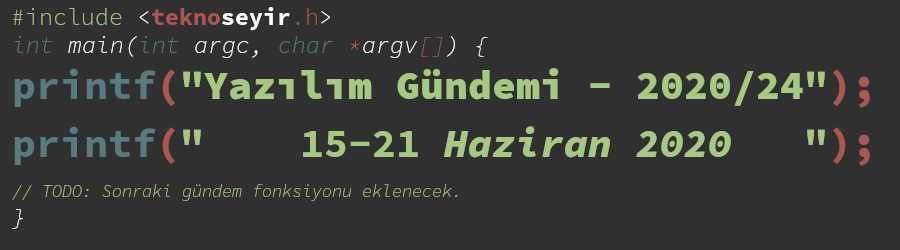
\includegraphics[width=.9\linewidth]{gorseller/yazilim-gundemi-banner.png}
\end{center}

\begin{center}
\href{../23/yazilim-gundemi-2020-23.pdf}{< Önceki Gündem} | \textbf{15-21 Haziran 2020} | \href{../25/yazilim-gundemi-2020-25.pdf}{Sonraki Gündem >}

\href{https://teknoseyir.com/blog/yazilim-gundemi-2020-24}{TeknoSeyir'de Oku}
\end{center}

\section{GitHub varsayılan branch ismini "main" \href{https://www.bbc.com/news/technology-53050955}{olarak değiştirecek}}
\label{sec:org3defc67}
Yaklaşık bir ay kadar önce ABD'de bir polisin siyahi bir vatandaşın ölümüne
yol açmasının ardından ortaya çıkan "Black Lives Matter" protestoları ucundan
kıyısından yazılım sektörünü de etkilemeye başlamıştı. Geçtiğimiz haftalarda
Google'ın Go projesi içerisindeki "master/slave" ve "blacklist/whitelist" gibi
ifadeleri kaldırığını haberleştirmiştim (bkz: \href{../22/yazilim-gundemi-2020-22.pdf}{Yazılım Gündemi - 2020/22}). Bu
hafta ise GitHub'ın benzer bir değişikliğe gideceğinin haberi aldık.

\begin{itemize}
\item \href{https://twitter.com/natfriedman/status/1271253144442253312}{Konuyla ilgili Tweet}
\end{itemize}

Hepimizin bildiği ve neredeyse her gün kullandığımız git versiyon kontrol
sisteminin varsayılan branch ismi olan "master" artık "main" olarak
değiştiriliyor. Bu dal ismini zaten kendimiz de değiştirebiliyorduk ama artık
GitHub'da oluşturduğunuz depoların varsayılan dal ismi "main" şeklinde
gelecek. Bunun nedeni olarak ise "master/slave" terminolojisi gösterilmiş.
Açıkcası bana bu neden biraz saçma geldi çünkü git versiyonlama sisteminde
"master/slave" ikilisi yok; sadece "master" terimi var o da ırkçı bir anlama
gelemeyecek kadar genel bir kullanım haline gelmiş durumda. Bu değişikliği
saçma bulan bir geliştirici de GitHub'ın bunu uygulamaması için \href{https://www.change.org/p/github-we-don-t-need-to-rename-the-master-branch-on-git}{Change
üzerinde bir imza kampanyası} başlatmış.

Aynı ve benzer değişikliklerin farklı projelerde (Örnek: \href{https://github.com/openssl/openssl/pull/12089}{openssl}) ve araçlarda
da yapılması gerektiğine yönelik birçok tartışma sektör içerisindeki çeşitli
platformlarda dönüyor. "blacklist/whitelist" ikilisinin "blocklist/allowlist"
olarak değiştirilmesini anlayabiliyorum; aynı şekilde "master/slave" ikilisini
kullanan projelerin de değiştirmesini anlıyorum ama \textbf{sadece "master"}
ifadesini kullanan GitHub'ın böyle bir değişikliğe neden gittiğini
anlayamıyorum. Sanırım "Ya herkes \emph{Black Lives Matter} ile ilgili PR çalışması
yapıyor, biz de böyle bi' şey yapalım, geri kalmayalım" diye düşünmüş
olabilirler. Açıkcası ben bu tarz yüzeysel şeyleri konuyu farklı noktaya çekme
çabası olarak görüyorum. Çünkü ırkçılık sorununun asıl kökenini bulma
amacından uzaklaştıran bir davranış. O zaman "üniversitede master yapmak"
ifadesi ya da ses terminolojisindeki "master" ifadesi de değiştirilsin yani
(!).

Bu konuda siz ne düşünüyorsunuz? Yorumlar bölümünde konulaşım.
\section{GitHub Super Linter \href{https://github.blog/2020-06-18-introducing-github-super-linter-one-linter-to-rule-them-all/}{tanıtıldı}}
\label{sec:org9dc3d6a}
Programlama yaparken özellikle de takım halinde çalışırken kodlarda belirli
bir standardı oturtmak önceden zaman alıcı olabiliyordu. Her ne kadar
günümüzde \emph{linter} araçları imdadımıza yetişse de onların da konfigürasyonu
ile uğraşmak yine süreci uzatıyor. Özellikle de birden çok programlama dilinin
kullanıldığı projelerde haliyle birden çok linter aracı kullanmak gerekiyor.
İşte bu ve benzeri duruma çözüm getirmek için GitHub'da, geçtiğimiz hafta
içerisinde \href{https://github.com/github/super-linter}{GitHub Super Linter} isimli açık kaynak projesini tanıttı. \href{https://github.com/features/actions}{GitHub
Action} üzerinden çalıştırabilen bir \emph{linter} aracı.

GitHub Super Linter, aslında isminden de anlaşılacağı gibi birden çok linter
aracını tek çatı altında toplayan, bunları çalıştıran ve sonuçlarını
raporlayan ve GitHub Action ile projenize kolay bir şekilde dahil
edebileceğiniz bir araç. Python, Ruby, JavaScript/TypeScript ve Go gibi
popüler programlama dillerinin yanında JSON, YAML, DockerFile ve CSS gibi
dosya formatlarını da destekliyor. Yalnız PHP için \texttt{phpcs} aracı ile bir
destek sunmamışlar. Belki bunu ben ekleyip pull request gönderebilirim.
Bakacağım buna.

\begin{figure}[htbp]
\centering
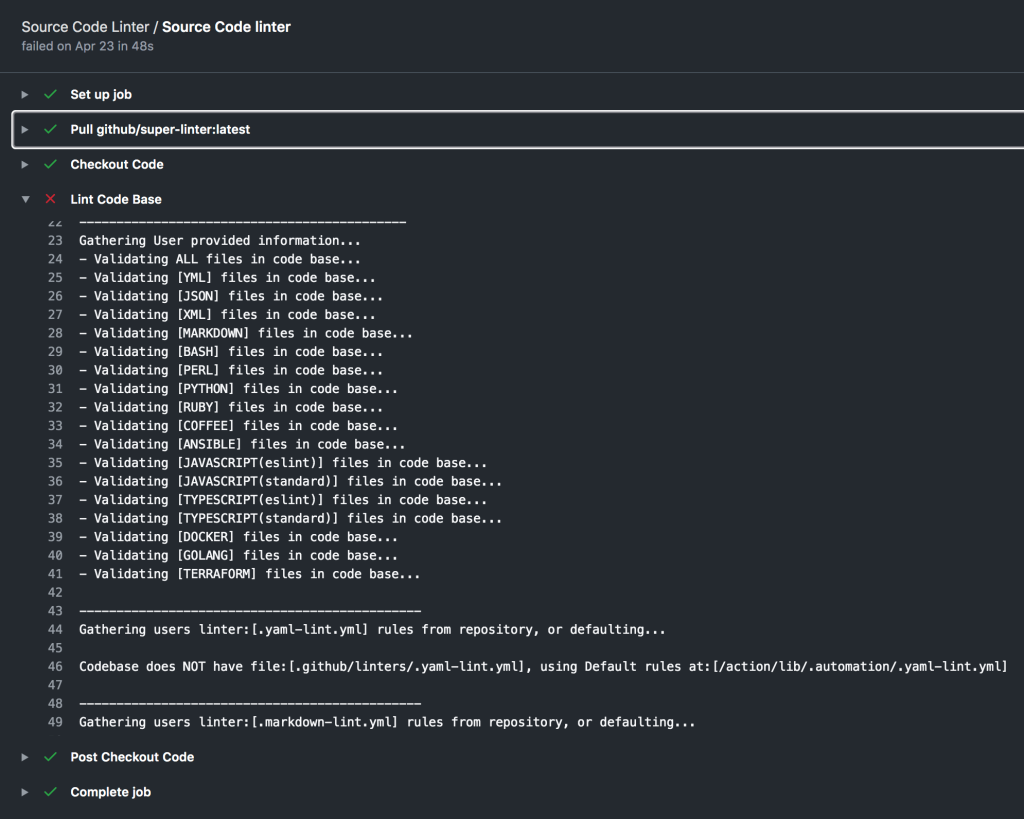
\includegraphics[height=7cm]{gorseller/github-super-linter.png}
\caption{Birçok programlama dili ve dosya formatı için linter çalıştırabiliyor}
\end{figure}
\newpage

GitHub Super Linter'in sağladığı bazı kolaylıklar ise şu şekilde:

\begin{itemize}
\item \texttt{master} vb. dallara çalışmayan kodların eklenmesini önleme
\item Birden çok programlama dili ile çalışırken kolayca kod standardı oluşturma
ve tüm projede kontrolleri sağlama
\item Code review süreçleri için otomatizasyon yardımı
\end{itemize}

GitHub'da depoladığınız projenize GitHub Action üzerinden çok kolay bir
şekilde ekleyip, istediğiniz diller ve dosya formatları için özelleştirmesini
yaparak aktifleştirebiliyorsunuz. Kullanımı ve özelleştirilmesiyle ilgili
diğer konular için \href{https://github.blog/2020-06-18-introducing-github-super-linter-one-linter-to-rule-them-all/}{şu GitHub deposunun README.md dosyasına} göz atabilirsiniz.
\section{Go dili topluluğu generic programlama özelliği için \href{https://blog.golang.org/generics-next-step}{yeni bir öneri yayınladı}: \href{https://go.googlesource.com/proposal/+/refs/heads/master/design/go2draft-type-parameters.md}{Type Parameters}}
\label{sec:org01b6b71}
İlk yazılım gündemi yazılarının birinde (bkz: \href{../../2019/04/yazilim-gundemi-04.pdf}{Yazılım Gündemi - 4}) Go dili
topluluğunun programlama diline generic programlama özellikleri eklemeyi
tartıştığını haberleştirmiştim. Geçtiğimiz hafta ise uzun bir aradan sonra bu
konuda ilk kez bir gelişme oldu ve Go takımı yeni bir öneriyi ("proposal")
tasarım taslağı olarak yayınladı. Dolayısıyla bunun henüz dile eklenmiş yeni
bir özellik ("feature") olmadığını ve üzerinde çeşitli değişikliklerin devam
edeceğini söylemekte fayda var.

Bu generic programlama özelliği için daha önce yayınlanan proposal'da
duyurulan \texttt{Contracts} yapısı artık terk edilmiş gözüküyor. Onun yerine gelen
tasarımsal değişiklik ise Type Parameters özelliği oldu. Kısaca bir örnek
yapmak gerekirse:
\begin{minted}[breaklines=true,breakanywhere=true,frame=lines, linenos, label=Go]{go}
func Print(type T)(s []T) {
  for _, v := range s {
    fmt.Println(v)
  }
}
\end{minted}

Yukarıda tanımladığımız fonksiyon kısaca herhangi bir türden diziyi alıp,
içerisindeki elemanları her biri bir satır olacak şekilde yazdırıyor. Yani
artık \texttt{int} dizisi için ayrı, \texttt{string} dizisi için ayrı fonksiyon yazmaya
gerek kalmıyor. Yukarıdaki fonksiyonun kullanımı ise şu şekilde:

\begin{minted}[breaklines=true,breakanywhere=true,frame=lines, linenos, label=Go]{go}
Print([]string{"Selam TeknoSeyir!", "Go generic programlama", "özelliğini deniyoruz.\n"})
Print([]int{1, 2, 3, 4, 5})
\end{minted}

\begin{figure}[htbp]
\centering
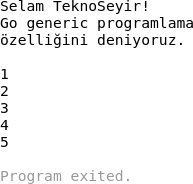
\includegraphics[height=3cm]{gorseller/go-generic-programlama.png}
\caption[\emph{/go2goplay.golang.org}]{Siz de bu özelliği test etmek isterseniz Go takımı tarafından hazırlanmış şu Playground sayfasını kullanabilirsiniz: \url{https://go2goplay.golang.org/}}
\end{figure}

Go takımı ve topluluğu özellik hakkında geri bildirimler toplamaya ve taslağı
geliştirmeye devam edecekler. Eğer bir aksilik olmazsa bu özelliği Ağustos
2021'de yayınlanması beklenen Go 1.17 sürümüyle birlikte stabil olarak
kullanabileceğiz.

Takım tarafından sunulan proposal sayfası acayip detaylı ve uzun bir sayfa,
benim de hepsini okumaya vaktim olmadığı için şimdilik bu kadar bilgi
verebiliyorum ama tabii ki dilerseniz detaylı bilgi ve kullanım örnekleri için
konu başlığına eklediğim bağlantılara tıklayabilirsiniz.
\section{Chromium takımının 2020 yılı \href{https://blog.chromium.org/2020/06/improving-chromiums-browser.html}{tarayıcı uyumluluğu çalışmaları}}
\label{sec:orgfc2cc57}
2019 yılında yayınlanan \href{https://insights.developer.mozilla.org/}{MDN Developer Needs Assessment} anketi sonuçlarından
sonra görüldü ki eskisi kadar olmasa da hâlâ daha web geliştiricilerin en
önemli sorunlarından birisi tarayıcılar arasındaki uyumsuzluk sorunları. Bu
bağlamda geçtiğimiz hafta içerisinde de Chromium takımı bir blog yazısı
yazarak 2020 yılı boyunca üzerinde çalışacakları uyumsuzluk sorunlarından ve
yaptıkları şeylerden bahsettiler.

Mart ayındaki bir yazılım gündemi yazısında (bkz: \href{../13/yazilim-gundemi-2020-13.pdf}{Yazılım Gündemi - 2020/13})
form elemanlarının stillerinin yenilendiğinden bahsetmiştim. Dolayısıyla bu
yazıya onu tekrar dahil etmiyorum. Sadece şöyle bir ekleme yapayım: Form
elemanlarının stillerinin güncellenmesine devam edilecekmiş. Bunun dışında
diğer konular ise şu şekilde:

\begin{itemize}
\item Flexbox ile ilgili uyumsuzluk sorunlarının üzerinde yoğun bir şekilde
çalışılıyormuş.
\item Flexbox ve CSS Grid özellikleri, takımın üzerinde çalıştığı yeni \href{https://www.chromium.org/blink/layoutng}{LayoutNG
arayüz motoru} ile yenilenecekmiş.
\item Scroll olayı ile ilgili de yeni uyumluluk çözümleri düşünülüyormuş fakat
tıkanılan, çözülmesi gereken bazı sorunlar varmış.
\end{itemize}

Çalışmalar ile ilgili daha detaylı bilgiler için konu başlığına eklediğim
bağlantıya tıklayabilirsiniz.
\section{Google, geliştiricilere uygulamayı yüklemeden \href{https://techcrunch.com/2020/06/17/google-is-launching-a-way-to-buy-android-app-subscriptions-outside-of-the-app-itself/}{abonelik satma imkanı sağlayacak}}
\label{sec:org40a7d9a}
Google'ın kendi Android işletim sistemiyle birlikte dağıttığı Play Store
mağaza uygulaması üzerinde artık kullanıcılar uygulamayı indirmeden de Google
üzerinden ilgili uygulamanın aboneliğini satın alabilecek. Geçtiğimiz hafta
Android 11'in yayınlanmasıyla birlikte sessizce duyurulan yeni \href{https://android-developers.googleblog.com/2020/06/meet-google-play-billing-library.html}{Google Play
Billing kütüphanesinin versiyon 3} sürümü buna izin veriyor.

Şimdilik sadece belirli birkaç geliştirici ve firmaya test olarak sunulmuş bu
özellik ile birlikte uygulamanın market sayfasında "Yükle" butonunun yanına
yeni bir "Abone ol ve yükle" butonu geliyor. Eğer uygulama birkaç günlük
ücretsiz bir teklif sunuyorsa "Free trials \& Install" yazabiliyor.

\begin{figure}[htbp]
\centering

\includegraphics[height=7.8cm]{gorseller/google-play-install.png}
\caption{Arayan ve SMS engelleme uygulaması Truecaller bu özelliği test edebilen uygulamalardan birisi.}
\end{figure}

Böylece artık kullanıcılarımız uygulamayı indirmeden de uygulama içerisinde
satılan uygulama-içi satın almalar hakkında bilgi alabiliyor ve dilerse Play
Store üzerinden bu işlemini gerçekleştirebiliyor olacak.

Diğer detaylar için konu başlığına eklediğim haber bağlantısına ya da
Google'ın yayınladığı blog yazısına bakabilirsiniz.
\section{Bootstrap \href{https://blog.getbootstrap.com/2020/06/16/bootstrap-5-alpha/}{5 Alpha yayınlandı}}
\label{sec:org4ba5b16}
Birçok back-end geliştiricinin kolayca uygulama çıkarabilmesini sağlamış ve bu
alandaki diğer arayüz framework'lerine de yol göstermiş olan Bootstrap v5
Alpha sürümü geçtiğimiz hafta içerisinde duyuruldu.

Bu sürümle birlikte artık jQuery terk edilmiş ve eski Internet Explorer
sürümleri için de destekler sonlanmış gözüküyor. Artık Bootstrap kullanırken
yanında bedava ve ekstra olarak gelen jQuery bağımlılığı yok. Yine de
jQuery'ye katkılarından dolayı teşekkür etmek gerek.

Internet Explorer desteğinin sonlandırılmasının bir getirisi olarak artık
Bootstrap 5 ile birlikte CSS üzerinde "Custom Properties" özelliğine sahip
olduk. Bu sayede artık CSS kodunun herhangi bir yerinde kullanabilmek üzere
değişkenler tanımlayabileceğiz. Örnek vermek gerekirse:
\begin{minted}[breaklines=true,breakanywhere=true,frame=lines, linenos, label=CSS]{css}
:root {
  --teknoseyir-kirmizisi: #ab1500;
  --beyaz: #fff;
}

.tekno {
  background-color: var(--beyaz);
  color: var(--teknoseyir-kirmizisi);
  /* */
}
\end{minted}
Artık bu yapıyı Bootstrap kendisi de elemanlarında kullanıyor.

Tabii ki bu sürümün Alpha etiketiyle yayınlandığını hatırlatmakta fayda var.
Yani henüz geçiş yapmak için çok erken. Yine de diğer detayları merak
ediyorsanız konu başlığına eklediğim bağlantıya tıklayabilirsiniz.
\section{Windows Terminal \href{https://devblogs.microsoft.com/commandline/windows-terminal-preview-1-1-release/}{Preview 1.1 sürümü yayınlandı}}
\label{sec:org2565e69}
Microsoft, geliştiricileri Windows ekosistemine çekmek için hamlelerine devam
ediyor. Geçtiğimiz hafta yayınlanan Windows Terminal Preview 1.1 sürümüyle
birlikte gelen özelliklerin bazıları şu şekilde:

\begin{figure}[htbp]
\centering
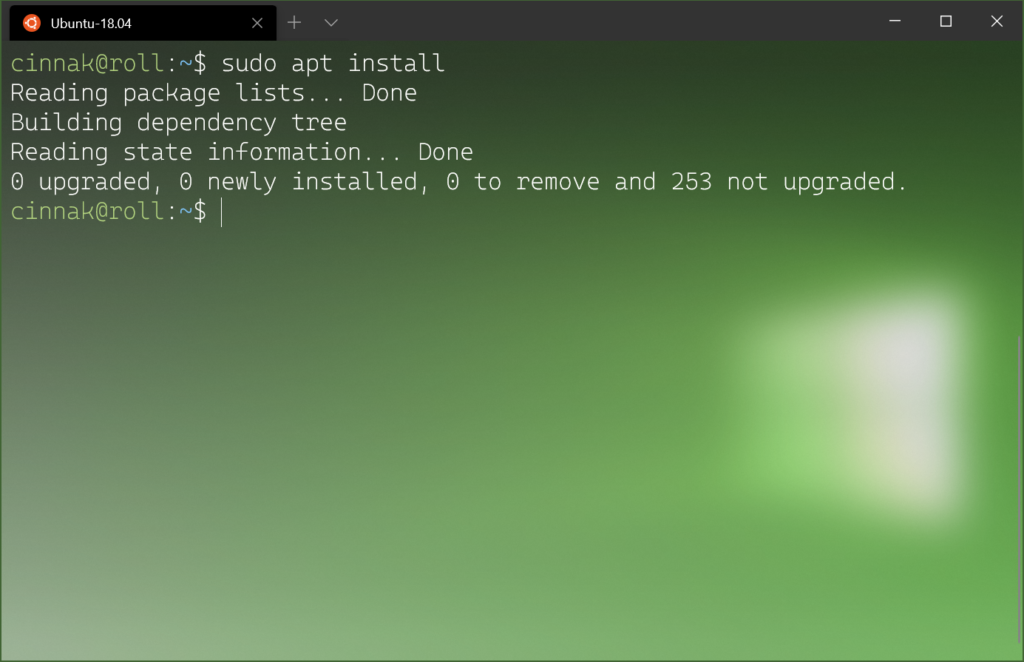
\includegraphics[width=.9\linewidth]{gorseller/winterm11-font-weight.png}
\caption[\texttt{"fontWeight": "normal"}]{Artık \texttt{"fontWeight": "normal"} gibi bir ifadeyi ayar dosyanıza ekleyerek terminal ekranındaki fontun kalınlığını ayarlabileceğiz. Tüm opsiyonlar için \href{https://docs.microsoft.com/en-us/windows/terminal/customize-settings/profile-settings\#text-settings}{buraya} bakabilirsiniz.}
\end{figure}
\newpage

Artık \texttt{Alt+Tıklama} kombinasyonunu aşağıdaki gibi kullanarak terminal
ekranımızı çoklu panellere bölebileceğiz.

\url{gorseller/winterm11-alt-tiklama.gif}

Bu sürümle birlikte Windows Terminal'in sekme özellikleri de gelişmiş durumda.
Artık sekmelerin isimleri değiştirebileceğiz ve onlara özel renkler
atayabileceğiz.

\begin{figure}[htbp]
\centering
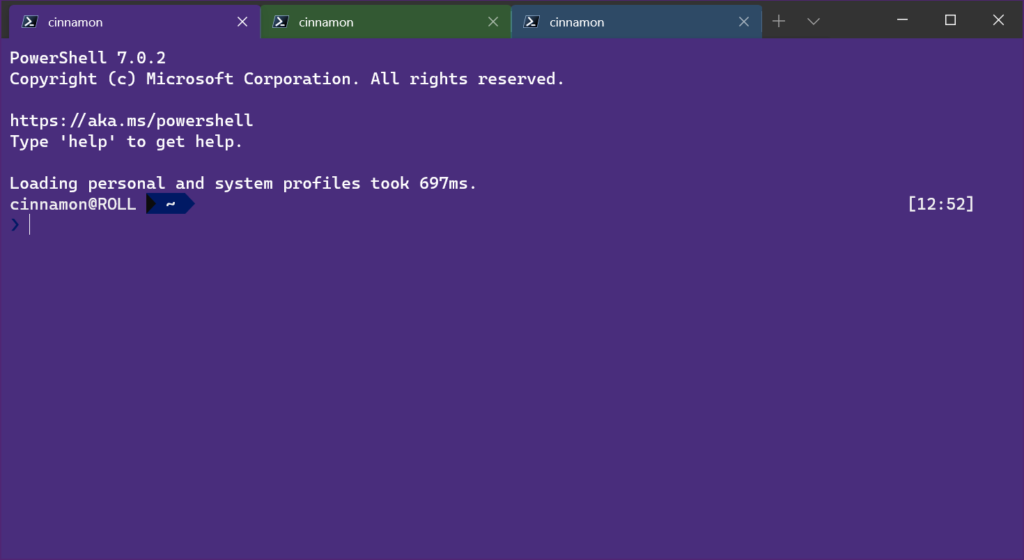
\includegraphics[width=.9\linewidth]{gorseller/winterm11-sekme-renk.png}
\caption{Sekmenin rengini değiştirmek için sağ tıklayıp, "Color\ldots{}" seçeneğine gelmek gerekiyor.}
\end{figure}
\newpage

\url{gorseller/winterm11-sekme-adlandir.gif}

Bunlara ek olarak artık komut satırını kullanarak yeni bir Windows Terminal
penceresi oluştururken iki yeni opsiyonumuz da var. İlki \texttt{-{}-maximized} ya da
\texttt{-M} ile yeni pencereyi ekranı kaplayacak şekilde oluşturabiliyoruz; ikincisi
ise \texttt{-{}-fullscreen} ya da \texttt{-F} ile yeni pencereyi tam ekran modunda
oluşturabiliyoruz. Ayrıca siz de benim gibi "Terminal benim yaşam ortamım
birçok şeyi orada yaparım" diyenlerdenseniz Windows 10'un açılışıyla birlikte
bir Windows Terminal penceresi açılsın istiyorsanız ayar dosyanıza aşağıdaki
satırı ekleyebilirsiniz:
\begin{minted}[breaklines=true,breakanywhere=true,frame=lines, linenos, label=JSON]{json}
"startOnUserLogin": true
\end{minted}

Her ne kadar GNU/Linux tarafına çoktan geçmiş bir geliştirici olsam da bu
gelişmelere Windows üzerinde çalışmak zorunda olan arkadaşlar için
seviniyorum. Mutlaka bir ara ben de deneyeceğim. Bakalım Microsoft ilerleyen
sürümlerde başka ne gibi özellikler gelecek.
\newpage
\section{Yaklaşan Online Etkinlikler}
\label{sec:org350fd03}
\begin{longtable}{|p{9.5cm}|l|}
\hline
Etkinlik İsmi & Tarihi\\
\hline
\endfirsthead
\multicolumn{2}{l}{Önceki sayfadan devam ediyor} \\
\hline

Etkinlik İsmi & Tarihi \\

\hline
\endhead
\hline\multicolumn{2}{r}{Devamı sonraki sayfada} \\
\endfoot
\endlastfoot
\hline
\href{https://kommunity.com/acmhacettepe/events/nodejs-deno-ve-js-ile-backend-gelistirmenin-dunu-ve-bugunu-eser-ozvataf-5ef2730a}{Eser Özvataf - Node.js, Deno ve JS ile Backend Geliştirmenin Dünü ve Bugünü} & 22 Haziran 21:00\\
\href{https://www.meetup.com/tr-TR/Microsoft-Giri\%25C5\%259Fimcilik-Bulu\%25C5\%259Fmalar\%25C4\%25B1/events/270863995/}{Developers Guide to AI} & 23 Haziran 11:00\\
\href{https://www.meetup.com/tr-TR/Microsoft-Giri\%25C5\%259Fimcilik-Bulu\%25C5\%259Fmalar\%25C4\%25B1/events/271151882/}{Building time machine with Event Sourcing} & 23 Haziran 17:00\\
\href{https://www.meetup.com/tr-TR/IBMDeveloperTR/events/270949885/}{Build a Secure App using S2I on Red Hat OpenShift} & 24 Haziran 14:00\\
\href{https://www.meetup.com/tr-TR/Teknolot/events/270951412/}{Build, integrate \& scale with event-driven apps} & 24 Haziran 14:00\\
\href{https://kommunity.com/cozumpark/events/teknoloji-sohbetleri-sanal-gerceklik-icin-yapay-zeka-ve-makine-ogrenimi-3cd4ca45}{Teknoloji Sohbetleri - Sanal Gerçeklik için Yapay Zeka ve Makine Öğrenimi} & 24 Haziran 14:00\\
\href{https://www.meetup.com/tr-TR/Microsoft-Giri\%25C5\%259Fimcilik-Bulu\%25C5\%259Fmalar\%25C4\%25B1/events/271152510/}{Azure Hybrid Virtual Event} & 24 Haziran 18:00\\
\href{https://www.meetup.com/tr-TR/Oracle-Developer-Meetup-Istanbul/events/271395295/}{More cloud native dev on OCI, with Functions, API, Streaming \{Events\} \& NoSQL} & 24 Haziran 18:00\\
\href{https://www.meetup.com/tr-TR/AWS-User-Group-Turkey/events/271307836/}{AWS Lambda \& Amazon API Gateway} & 24 Haziran 18:30\\
\href{https://kommunity.com/cloud-and-serverless-turkey/events/devopsdays-online-turkiye-2020-130a646d}{DevOpsDays Online Türkiye 2020} & 25 Haziran 08:30\\
\href{https://www.meetup.com/tr-TR/IBMDeveloperTR/events/271222367/}{Cloud Native Security Conference} & 25 Haziran 11:00\\
\href{https://www.meetup.com/tr-TR/Microsoft-Giri\%25C5\%259Fimcilik-Bulu\%25C5\%259Fmalar\%25C4\%25B1/events/271152397/}{Data \& AI Virtual Summit - Artificial Intelligence Track} & 25 Haziran 11:00\\
\href{https://www.meetup.com/tr-TR/IBMDeveloperTR/events/270925205/}{Watson Discovery with Node-Red on IBM Cloud} & 25 Haziran 14:00\\
\href{https://www.meetup.com/tr-TR/Istanbul-KNIME-Users/events/271392949/}{Text Mining Techniques} & 25 Haziran 19:00\\
\href{https://www.meetup.com/tr-TR/Hepsitech-Meetup/events/271247034/}{Test Automation - Robot Framework} & 25 Haziran 19:00\\
\href{https://www.meetup.com/tr-TR/Turkish-AI-Hub/events/271391778/}{Mozilla TTS ve Yapay Zeka Konuşma Sentezi} & 25 Haziran 20:30\\
\href{https://kommunity.com/bilge-adam-teknoloji/events/nodejs-ve-mongodb-kullanarak-uygulama-gelistirme-4e46c1ca}{Node.js ve MongoDB Kullanarak Uygulama Geliştirme} & 25 Haziran 21:00\\
\href{https://www.meetup.com/tr-TR/IBMDeveloperTR/events/270949799/}{Deploy a Cloud-Native Application on Red Hat OpenShift} & 26 Haziran 16:00\\
\href{https://kommunity.com/bilge-adam-teknoloji/events/html-css-ve-javascript-ile-web-arayuz-uygulamasi-1f18a563}{HTML, CSS ve JavaScript ile Web Arayüz Uygulaması} & 26 Haziran 19:15\\
\href{https://www.meetup.com/tr-TR/GDGAnkara/events/271395414/}{Flutter Day} & 27 Haziran 16:00\\
\hline
\end{longtable}
\section{Diğer Haberler}
\label{sec:org0edf5ef}
\begin{itemize}
\item Almanya kendi koronavirüs takip uygulamasını \href{https://github.com/corona-warn-app/cwa-documentation}{açık kaynak yaptı}.
\item Microsoft, Windows Subsystem for Linux'a \href{https://blogs.windows.com/windowsdeveloper/2020/06/17/gpu-accelerated-ml-training-inside-the-windows-subsystem-for-linux/}{NVDIA CUDA desteği ekledi}.
\item Google Cloud, yeni bir depolama \href{https://techcrunch.com/2020/06/16/google-cloud-launches-filestore-high-scale-a-new-storage-tier-for-high-performance-computing-workloads/}{seçeneğini duyurdu}: \href{https://cloud.google.com/filestore/docs/high-scale}{Filestore High Scale}.
\item Araştırmacılar Kuantum bilgisayarlar için ilk \href{https://ethz.ch/en/news-and-events/eth-news/news/2020/06/the-first-intuitive-programming-language-for-quantum-computers.html}{programlama dilini
geliştirdiler}: \href{https://silq.ethz.ch/}{Silq}.
\item OpenAI organizasyonu yeni \href{https://openai.com/blog/image-gpt/}{çalışmasını duyurdu}: Image GPT.
\item .NET için gRPC-Web \href{https://devblogs.microsoft.com/aspnet/grpc-web-for-net-now-available/}{yayınlandı}. \href{https://github.com/grpc/grpc-dotnet}{GitHub Deposu}
\item AdoptOpenJDK projesi \href{https://blog.adoptopenjdk.net/2020/06/adoptopenjdk-to-join-the-eclipse-foundation/}{Eclipse Foundation'a katıldı}.
\item Eclipse IDE \href{https://www.eclipse.org/eclipse/news/4.16/}{2020-06 (v4.16) sürümü yayınlandı}.
\item Free Pascal \href{https://wiki.freepascal.org/FPC\_New\_Features\_3.2.0\#About\_this\_page}{3.2.0 sürümü yayınlandı}.
\item Apache Spark \href{https://spark.apache.org/releases/spark-release-3-0-0.html}{3.0.0 sürümü yayınlandı}.
\item TiDB \href{https://pingcap.com/blog/tidb-4.0-ga-gearing-you-up-for-an-unpredictable-world-with-real-time-htap-database/}{4.0 GA sürümü yayınlandı}.
\item OpenAPI \href{https://www.openapis.org/blog/2020/06/18/openapi-3-1-0-rc0-its-here}{3.1.0 sürümü yayınlandı}.
\item RestClient.Net \href{https://christianfindlay.com/2020/06/17/restclient-net-4-0/}{4.0 sürümü yayınlandı}.
\end{itemize}
\section{Lisans}
\label{sec:org5684c08}
\begin{center}
\begin{center}

\includegraphics[height=1.5cm]{../../../img/CC_BY-NC-SA_4.0.png}
\end{center}

\href{yazilim-gundemi-2020-24.pdf}{Yazılım Gündemi - 2020/24} yazısı \href{https://erenhatirnaz.github.io}{Eren Hatırnaz} tarafından \href{http://creativecommons.org/licenses/by-nc-sa/4.0/}{Creative Commons
Atıf-GayriTicari-AynıLisanslaPaylaş 4.0 Uluslararası Lisansı} (CC BY-NC-SA 4.0)
ile lisanslanmıştır.
\end{center}
\end{document}
